\documentclass[../main.tex]{subfiles}

\begin{document}

\justifying

\section{Directory: 2026-02-05-140904}

\paragraph{Objetivo} Analizar la tabulación del potencial de interacción entre patches $U_\mathrm{patch}$ en LAMMPS.

\subsection{Simulation description}

Se coloca una partícula en el centro de la caja de simulación, \(\vec{r}_1 = (0,0,0)\).
Se coloca una segunda partícula a una distancia de \num{0.75} de la partícula central, \(\vec{r}_2 = (-0.75,0,0)\).
Usando el comando \verb|fix move| se mueve la segunda partícula a velocidad constante de \num{0.1}, \(\vec{v}_2 = (0.1,0,0)\), hacia el centro de la caja.
El paso temporal es de \num{1d-3}.
El número de pasos es \num{4500}, obteniendo una simulación de \num{4.5} unidades temporales.

\subsection{Resultados}

\begin{figure}[ht]
    \centering
    
\includegraphics[width=\textwidth]{../Figures/2026-02-05-140904/fig_comp.png}
    \caption{Evolución temporal de las componentes de la posición de cada una de las partículas.
    En el panel superior es la componente $x$ de cada partícula y en el panel inferior es la componente $y$ de cada partícula a lo largo de la simulación.}\label{fig:1_componentes}
\end{figure}

\newpage

\begin{figure}[ht]
    \centering
    
\includegraphics[width=0.8\textwidth]{../Figures/2026-02-05-140904/fig_pot.png}
    \caption{Evolución temporal de la energía potencial en cada partícula y la evolución temporal de la distancia entre partículas.
    En el panel de arriba es la evolución temporal de la partícula qué está en el centro y en el panel de abajo es la evolución temporal de la energía potencial de la partícula que se está acercando.
    En el panel de en medio es la evolución temporal de la distancia entre partículas.}\label{fig:2_Upotpart}
\end{figure}

\hfill

\begin{figure}[ht]
    \centering
    
\includegraphics[width=0.8\textwidth]{../Figures/2026-02-05-140904/fig_potComp.png}
    \caption{Comparación de la energía potencial entre la simulación y la forma algebráica.
    \(U_{\mathrm{sim}}\) es la energía potencial que da LAMMPS.
    \(U_{\mathrm{eval}}\) es la energía potencial que sale de evaluar el potencial con la distancia obtenida a través de los datos de la simulación.
    \(U_{\mathrm{ref}}\) es el potencial de interacción evaluado con un dominio creado a parte.}\label{fig:3_UpotComp}
\end{figure}


\newpage

\subsection{Comentarios/Análsis}

\ldots Éxito parcial? 
En términos generales, por la figura \ref{fig:3_UpotComp} se puede decir que la tabulación está parcialmente correcta.
Tiene la forma del pozo potencial, pero el pozo de potencial es mayor con respecto a la definición.

Lo que no logro comprender, son los datos que encuentro en el \verb|dump|.
Creando un zoom de la figura \ref{fig:1_componentes} en las primeras iteraciones (\ref{fig:4_componentes}) podemos obeservar que la partícula \emph{regresa} periódicamente a valores cercanos a su posición original.
No entiendo porque hace eso.

\begin{marginfigure}
    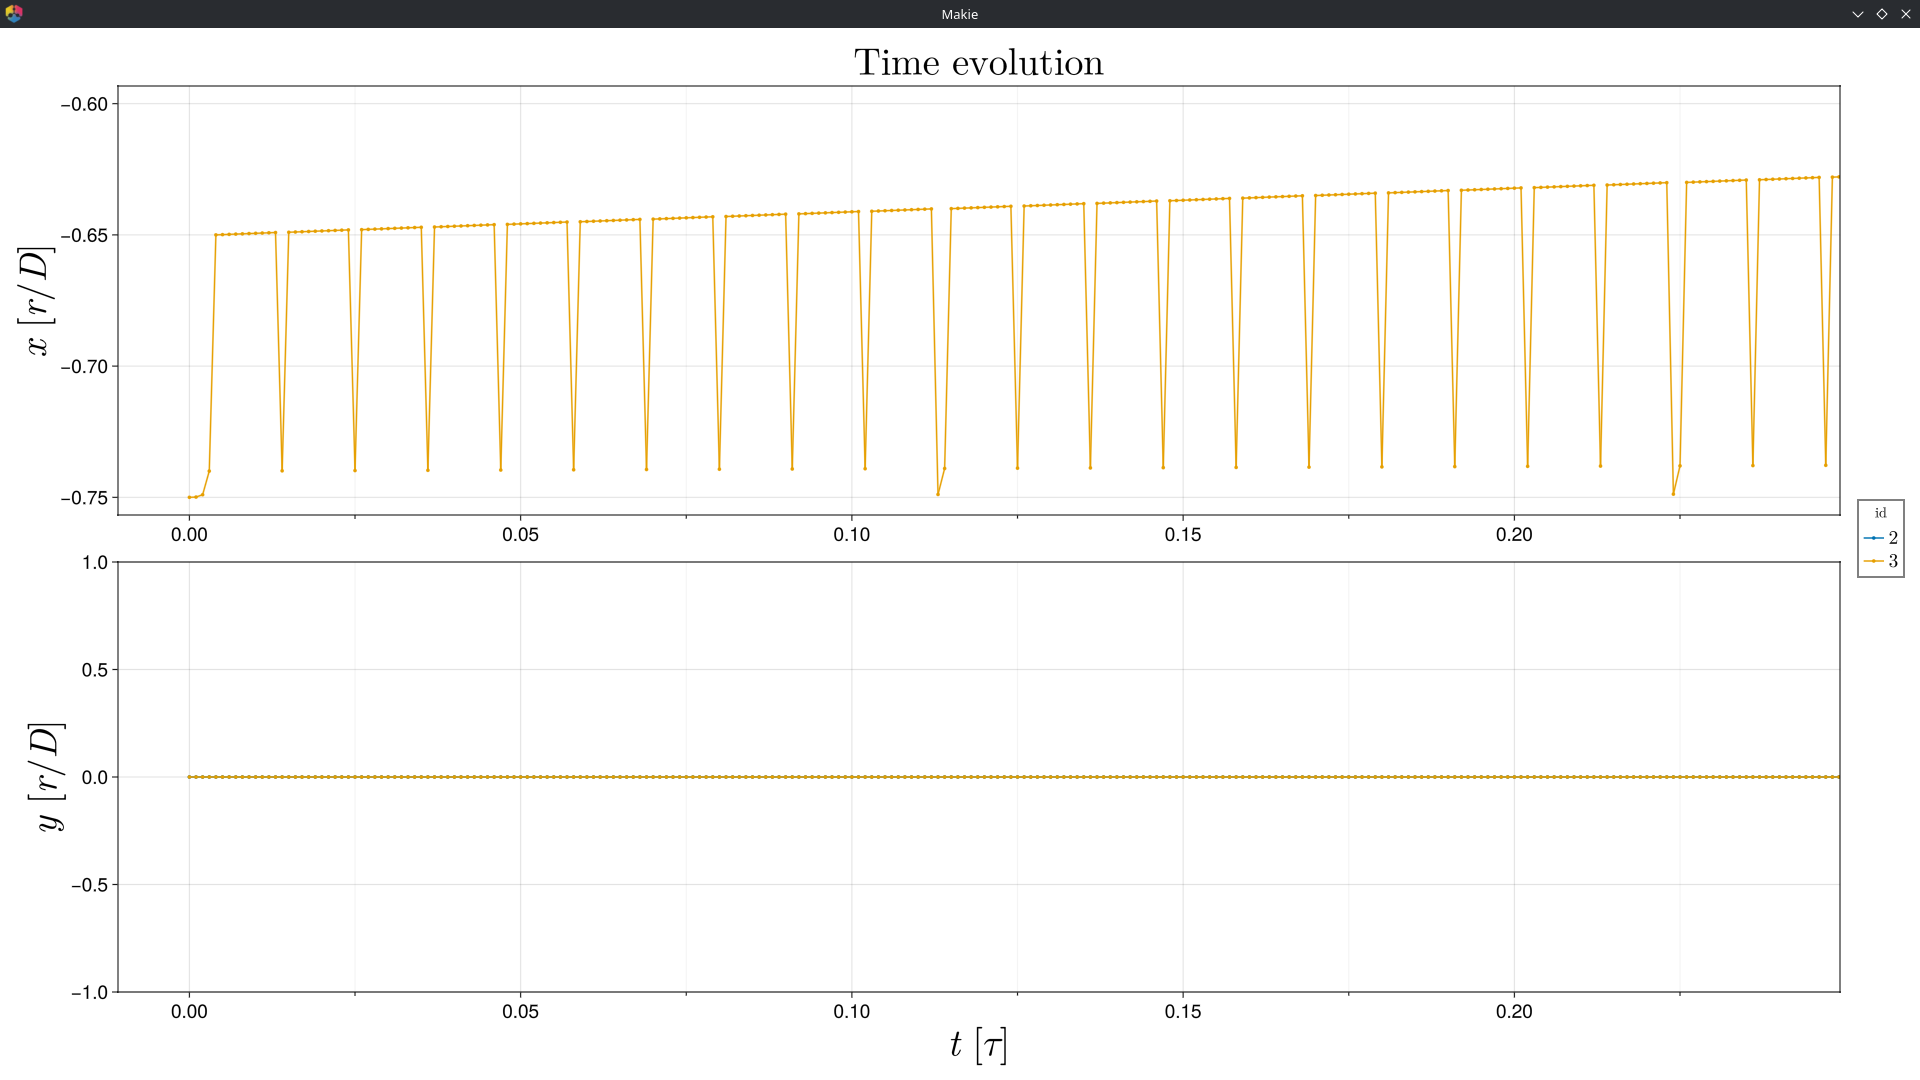
\includegraphics[width=\textwidth]{../Figures/2026-02-05-140904/fig_comp_zoom.png}
    \caption{Acercamiento de la figura~\ref{fig:1_componentes}.}\label{fig:4_componentes}
\end{marginfigure}

El código que configura el movimiento está declarado de la siguiente manera:
\begin{code}
# RUN SIMULATION
timestep ${tstep}
fix movePA PAm move linear 0.1 0.0 0.0
run ${steps}
\end{code}
Fin.

Peor aún, en la figura~\ref{fig:1_componentes}, por el segundo $\approx$\num{3.8} hay una discontinuidad que no sé porque está.
Lo peor de todo es que cuando analizo la información del \verb|dump| en ovito, parece que todo va bien: \href{https://youtu.be/L48lPIuFl4U}{https://youtu.be/L48lPIuFl4U}
\begin{marginfigure}
    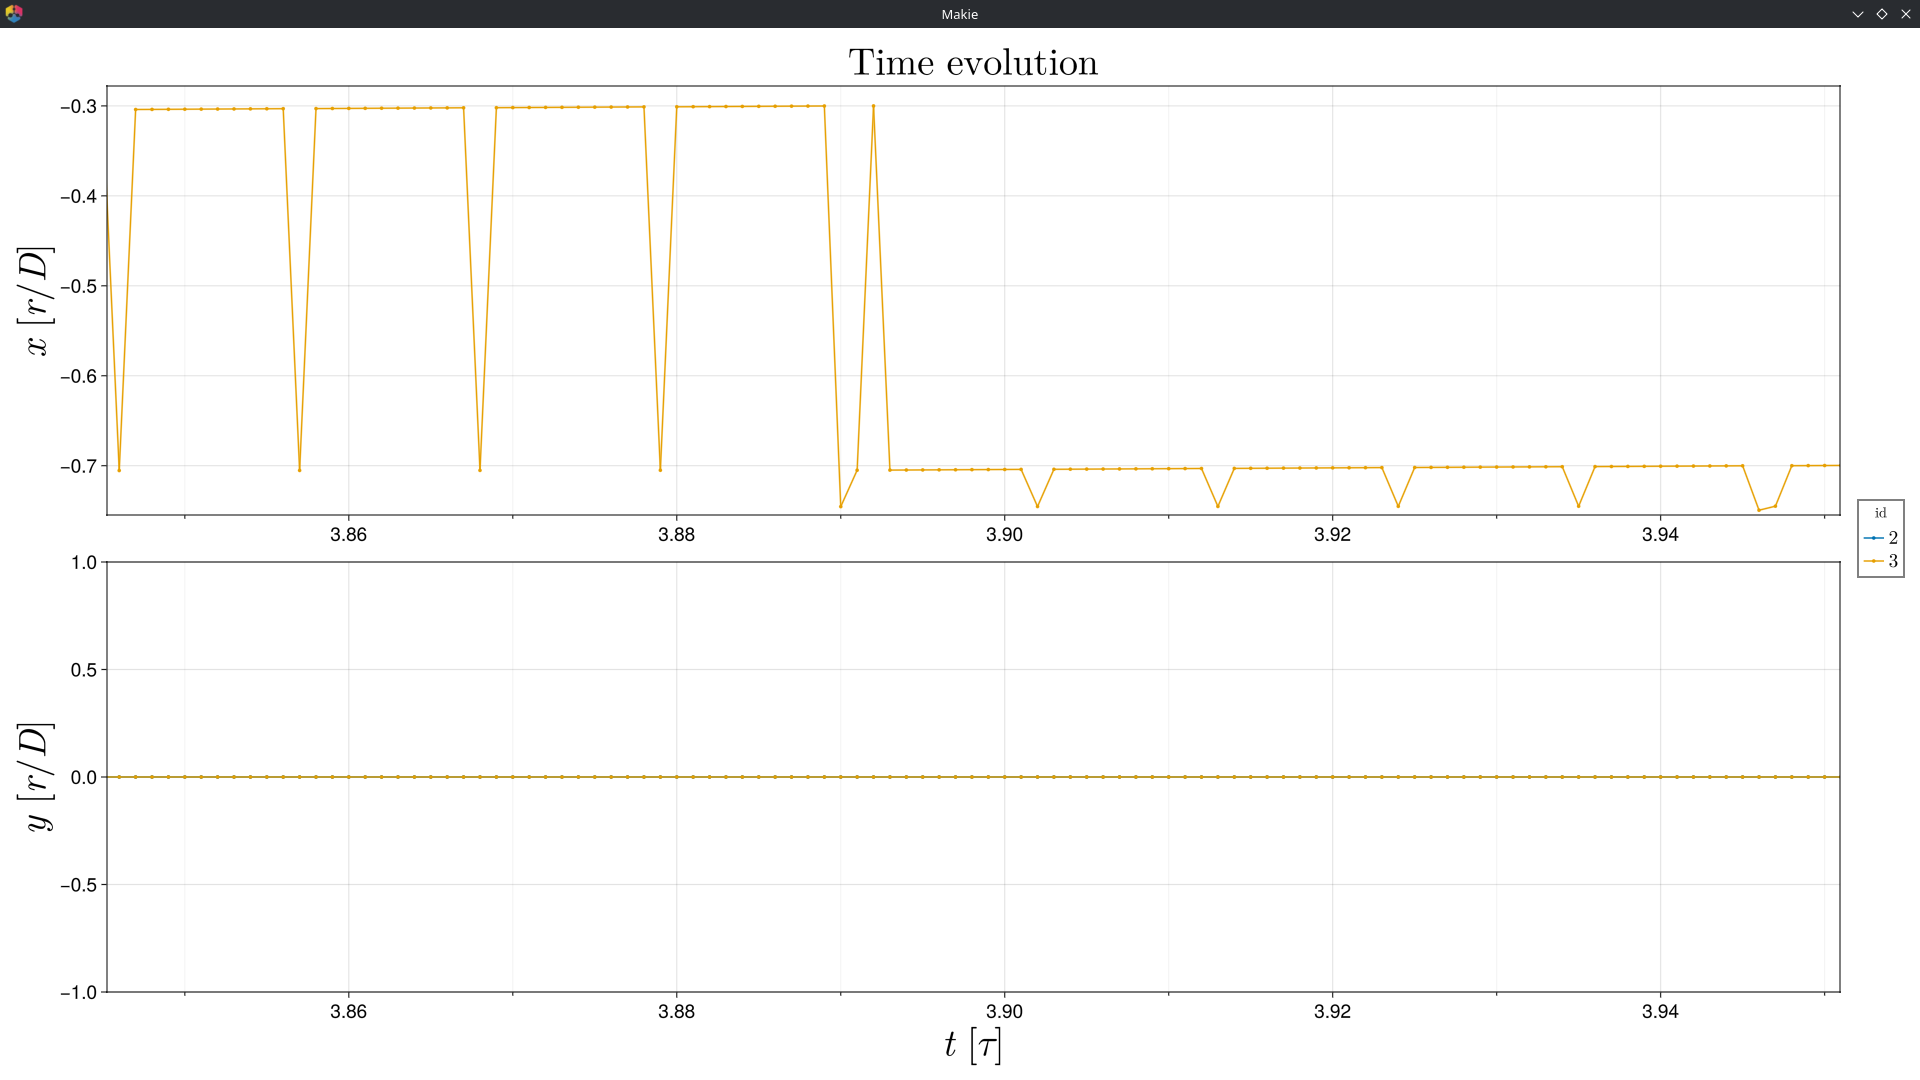
\includegraphics[width=\textwidth]{../Figures/2026-02-05-140904/fig_comp_zoom_2.png}
    \caption{Acercamiento de la figura~\ref{fig:1_componentes}.}\label{fig:5_componentes}
\end{marginfigure}

Viendo con calma, el error está en cómo estoy procesando los archivos \verb|dump|.



\end{document}
